\documentclass[12pt,times,a4paper,twoside]{article}

\usepackage[utf8]{inputenc}	% Para caracteres en español
\usepackage[left=3cm,right=3cm,top=2cm,bottom=3cm]{geometry}
\usepackage{pagenote}

\usepackage{algorithm}
\usepackage{algorithmic}

\usepackage{amsmath,amsthm,amsfonts,amssymb,amscd}
\usepackage{mathtools,xparse}
\usepackage{mathrsfs}

\usepackage{multirow,booktabs}
\usepackage[table]{xcolor}
\usepackage{fullpage}
\usepackage{lastpage}
\usepackage{enumitem}
\usepackage{fancyhdr}

\usepackage{graphicx}
\usepackage{wrapfig}
\usepackage{setspace}
\usepackage{calc}
% \usepackage{color,soul}
\usepackage{multicol}
\usepackage{cancel}
\usepackage[retainorgcmds]{IEEEtrantools}
% \usepackage{xcolor} -- implied by xcolor

\usepackage{listings}
\usepackage{spverbatim}
\usepackage{fancyvrb}
\usepackage{hyperref}
\usepackage{float} 
\usepackage{natbib}

\usepackage{tikz}
\usepackage{pgfplots}
\usepackage{pgfplotstable}

\usepackage{soulutf8}
\usepackage{tabularx}

\usepackage{multirow}
\usepackage{adjustbox}
\usepackage{caption}
\usepackage{subcaption}

\usepackage[draft]{todo}
\newcommand{\fyTodo}[1]{\Todo[FY:]{\textcolor{orange}{#1}}}
\newcommand{\fyTodostar}[1]{\Todo*[FY:]{\textcolor{orange}{#1}}}
\newcommand{\fyDone}[1]{\done[FY]\Todo[FY:]{\textcolor{orange}{#1}}}
\newcommand{\fyDonestar}[1]{\done[FY]\Todo[FY:]{\textcolor{orange}{#1}}}
\newcommand{\domain}[1]{\texttt{\textsc{#1}}}
\newcommand{\system}[1]{\texttt{{#1}}}
\colorlet{shadecolor}{orange!15}
\parindent 0in
\parskip 12pt
\geometry{margin=1in, headsep=0.25in}
\setlength{\belowdisplayskip}{8pt} \setlength{\belowdisplayshortskip}{8pt}
\setlength{\abovedisplayskip}{8pt} \setlength{\abovedisplayshortskip}{8pt}
\setlist{nosep}
\setlength{\parskip}{0.1cm}
\setlength{\parindent}{1em}

\theoremstyle{definition}
\newtheorem{defn}{Definition}
\newtheorem{lemma}{Lemma}[section]
\newtheorem{theorem}{Theorem}[section]
\newtheorem{proposition}{Proposition}[section]
\newtheorem{definition}{Definition}[section]
\DeclareMathOperator*{\argmax}{argmax}
\newcommand{\R}{\ensuremath{\mathbb{R}}}

\pgfkeys{
    /tr/rowfilter/.style 2 args={
        /pgfplots/x filter/.append code={
            \edef\arga{\thisrow{#1}}
            \edef\argb{#2}
            \ifx\arga\argb
            \else
                \def\pgfmathresult{}
            \fi
        }
    }
}

\DeclarePairedDelimiter{\abs}{\lvert}{\rvert}
\DeclarePairedDelimiter{\norm}{\lVert}{\rVert}
\NewDocumentCommand{\normL}{ s O{} m }{%
  \IfBooleanTF{#1}{\norm*{#3}}{\norm[#2]{#3}}_{L_1}%
}

\title{MDMT training}
\author{}
\date{}

\begin{document}
\maketitle

\section{Results}
\subsection{Variants of the original algorithm}
We have found 3 variants of the algorithm which lead to a significant change in the behavior of the algorithm. Those 3 options are the number of updates before computing gradient over validation sets that we denote $sim\_iter$; the parameterization of the sampling distribution; and the regularization on sampling distribution (we chose entropy maximization as regularizing method). We report the performance of the resulting models in table \ref{tab:performance} and the sampling distribution of the domains in figure \ref{fig:sampling}

\begin{table}
  \centering% \small
  \begin{adjustbox}{width=1.0\columnwidth,center}
  \begin{tabular}{|p{3.0cm}|*{13}{r|}} \hline
    \multirow{2}{*}{Name} & \multirow{2}{*}{$sim\_iter$} & \multirow{2}{*}{parameterization} & \multirow{2}{*}{entropy constraint} & \multicolumn{6}{|c|}{BLEU} & \multirow{2}{*}{BLEU average} \\ \cline{5-10}	
   & & & & \multicolumn{1}{c|}{\domain{ med}} & \multicolumn{1}{c|}{\domain{ law}} & \multicolumn{1}{c|}{\domain{bank}} & \multicolumn{1}{c|}{\domain{talk}} & \multicolumn{1}{c|}{\domain{ it }} & \multicolumn{1}{c|}{\domain{ rel}} &  \\
    \hline
  \system{$config\_673$} & 10 & linear & yes & 36.02& 56.18& 52.96& 32.06& 45.2 & 90.94 & 52.23 \\
  \system{$config\_675$} & 10 & softmax & yes & 36.24& 55.67& 52.63& 32.74& 44.47& 90.45& 52.03\\
  \system{$config\_616$} & 1 & softmax & yes & 36.96& 55.55& 52.88& 33.06& 44.52& 91.25& 52.37 \\
  \system{$config\_603$} & 1 & softmax & no & 37.26& 55.07& 50.96& 33.49& 43.41& 90.76& 51.83\\
  \hline
  \end{tabular}
  \end{adjustbox}
  \caption{BLEU over multi-domain test sets}
  \label{tab:performance}
\end{table}

\begin{figure}[htb]
\begin{subfigure}{.5\textwidth}
  \centering
  % include first image
  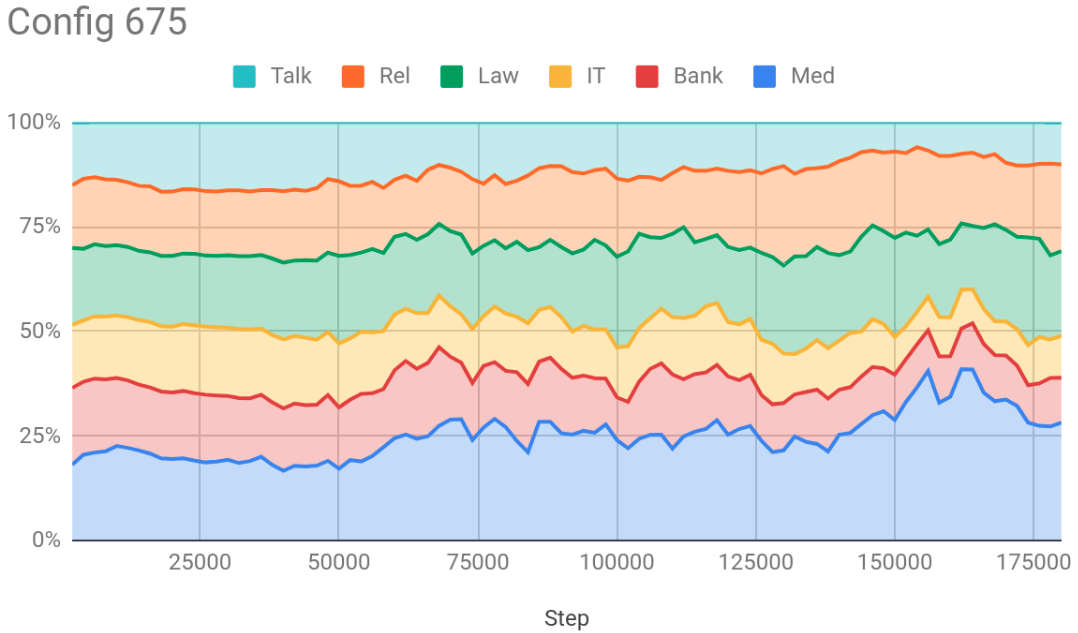
\includegraphics[width=.8\linewidth]{config675.png}  
  \caption{config 675}
  \label{fig:675}
\end{subfigure}
\begin{subfigure}{.5\textwidth}
  \centering
  % include second image
  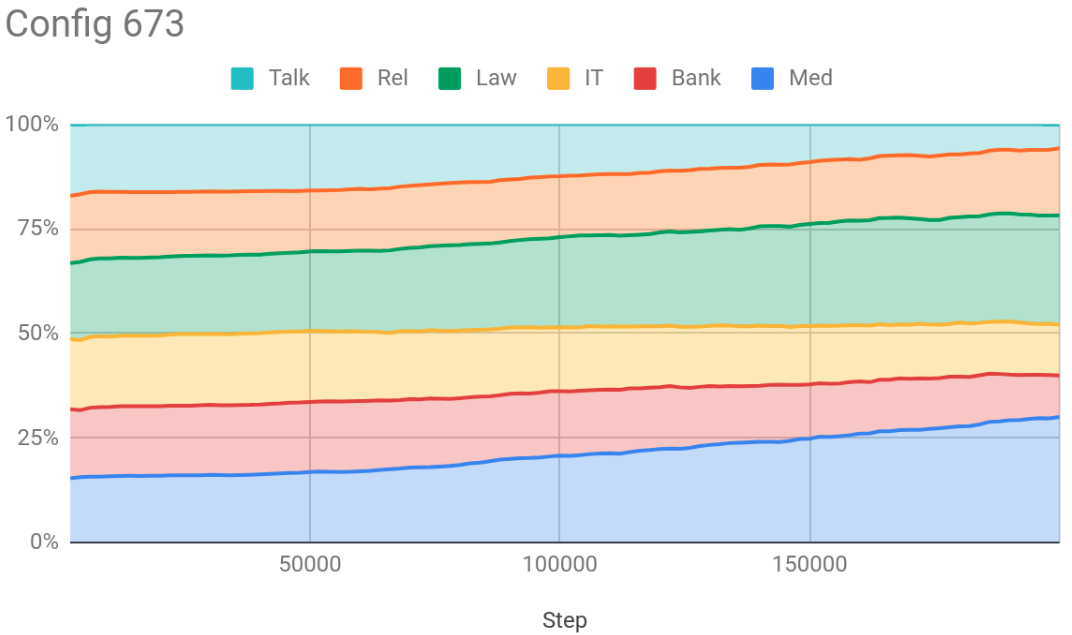
\includegraphics[width=.8\linewidth]{config673.png}  
  \caption{Config 673}
  \label{fig:673}
\end{subfigure}
\newline
\begin{subfigure}{.5\textwidth}
  \centering
  % include third image
  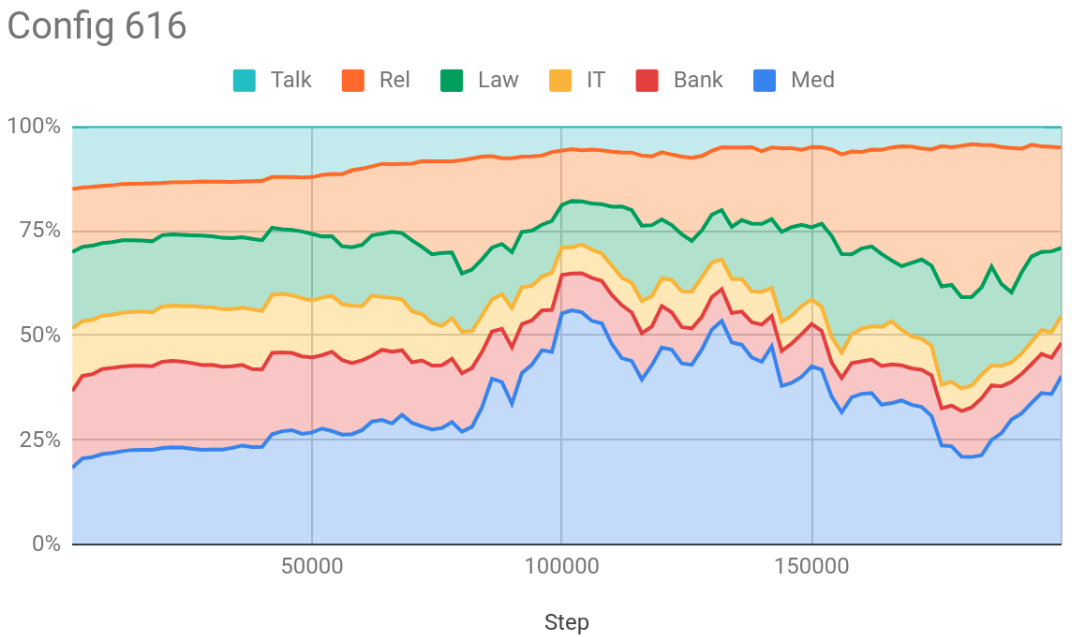
\includegraphics[width=.8\linewidth]{config616.png}  
  \caption{Config 616}
  \label{fig:616}
\end{subfigure}
\begin{subfigure}{.5\textwidth}
  \centering
  % include fourth image
  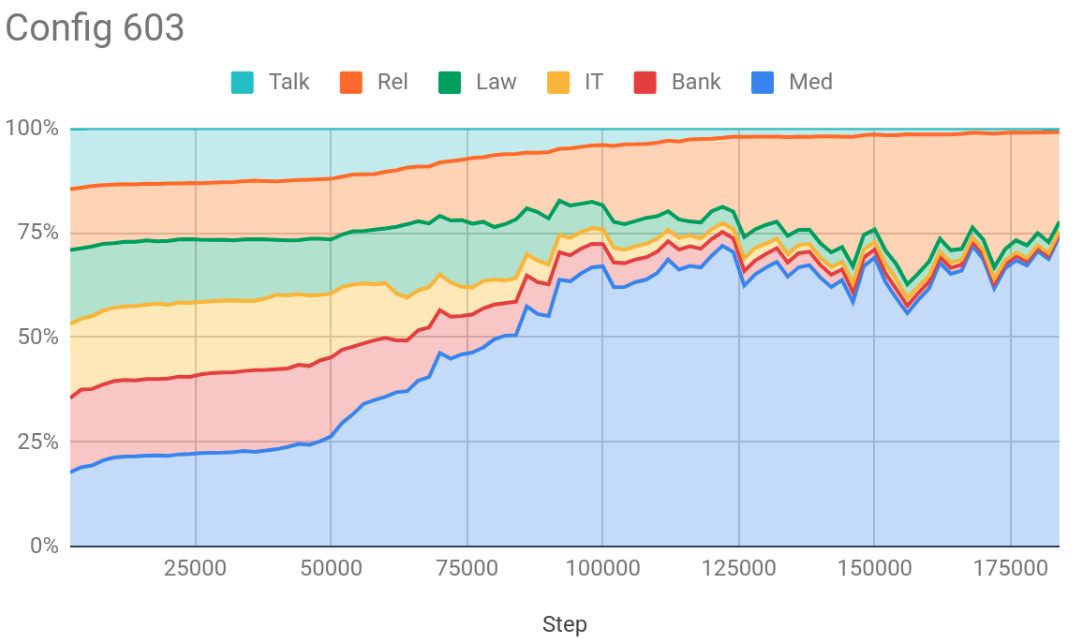
\includegraphics[width=.8\linewidth]{config603.png}  
  \caption{Config 603}
  \label{fig:603}
\end{subfigure}
\caption{Sampling distribution}
\label{fig:sampling}
\end{figure}

Changing the number of updates (denoted $sim\_iter$) before computing gradient over the validation sets can be interpreted as a simple approximation of an extension of the original optimization problem. We recall that the sampler's parameter $\psi$ is optimized to reduce the following loss:

\begin{align*}
L(\theta^t,\psi) &=  \displaystyle{\mathop{\sum_{i=1}^k}} L(\theta^{t+1}, Q^{dev}_i) \\
\theta^{t+1} &= \theta^{t+i} - \eta * \frac{\partial l(\theta_{t+i}, x^i,y^i)}{\partial \theta} \\
x^i,y^i &\sim Q^{trn}(\psi)
\end{align*}

We extend the problem to further evaluation point $t+N$ instead of $t+1$ in the training course

\begin{align*}
L(\theta^t,\psi) &=  \displaystyle{\mathop{\sum_{i=1}^k}} L(\theta^{t+N}, Q^{dev}_i) \\
\theta^{t+i+1} &= \theta^t - \eta * \frac{\partial l(\theta_{t+i}, x,y)}{\partial \theta} \forall 0 \leq i \leq N-1\\
x,y &\sim Q^{trn}(\psi)
\end{align*}

By comparing figure \ref{fig:616} and \ref{fig:675} we observe that changing $sim\_iter$ leads to a significant shift in the resulting sampling distribution in which \domain{rel} is reduced while other domains become more frequent.

The second variant is the parameterization of the sampling distribution. We've found that optimizing softmax parameterization without regularization usually leads to a critical point in which one or two domains take all percentages while other domains disappear. Furthermore, the gradient $\psi_i$ in the softmax parameterization has closed-form as follow
\begin{align*}
\frac{\partial l}{\partial \psi_i} & = \displaystyle{\mathop{\sum}_{j=1}^K} R_j \frac{\partial P_j}{\partial \psi_i} \\
	& = R_i P_i*(1-P_i) - \displaystyle{\mathop{\sum}_{j\neq i}^K} R_j P_j P_i \\
	& = P_i(R_i-l)\\
\end{align*} 
which is proportional to the current value $p_i$, which will lead to the "richer get richer" phenomenon. By comparing figure \ref{fig:603} and \ref{fig:673}, we observe that the severe drop in the poor domains is reduced by replacing softmax parameterization with linear parameterization which uses the following updates

\begin{align*}
\psi_i = \frac{\psi_i + \eta * R_i}{ 1 + \eta \displaystyle{\mathop{\sum}_{j=1}^K} R_j}
\end{align*}

Finally, as we forementioned in the previous paragraph, to slow down the phenomenon "richer gets richer", we use entropy maximizing to regularize the sampling distribution, which leads to a better optimal distribution that does not discard poor domains which may be "prematurely" misjudged.

\subsection{Domain adaptation with less catatrophic forgetting}
DDS method could perform domain adaptation by down-weighing the contribution of domains other than the target-domain in the evaluation score to 0. We report fine-tuned systems using the DDS method, $DDS\_FT\_\{ med, bank, law, IT, rel, talk \}$. We report the performances of those systems in the table \ref{tab:ft}. We observe that out-of-interest domains do not lose huge performance as usually reported in the standard fine-tuning method. \fyTodo{to compare with mixed domain adaptation of Dabre}.

\begin{table}[htb]
  \centering% \small
  \begin{adjustbox}{width=1.0\columnwidth,center}
  \begin{tabular}{|p{3.0cm}|*{13}{r|}} \hline
    \multirow{2}{*}{Name} & \multirow{2}{*}{$sim\_iter$} & \multirow{2}{*}{parameterization} & \multirow{2}{*}{entropy constraint} & \multicolumn{6}{|c|}{BLEU} & \multirow{2}{*}{BLEU average} \\ \cline{5-10}	
   & & & & \multicolumn{1}{c|}{\domain{ med}} & \multicolumn{1}{c|}{\domain{ law}} & \multicolumn{1}{c|}{\domain{bank}} & \multicolumn{1}{c|}{\domain{talk}} & \multicolumn{1}{c|}{\domain{ it }} & \multicolumn{1}{c|}{\domain{ rel}} &  \\
    \hline
  \system{$DDS\_FT\_med$} & 1 & softmax & no & 36.7&51.14&52&44.32&90.41&33.22&51.3\\
  \system{$DDS\_FT\_law$} & 1 & softmax & no &36.05&56.18&53.57&44.05&91.24&33.09&52.36\\
  \system{$DDS\_FT\_bank$} & 1 & softmax & no &36.15&54.17&54.29&41.33&89.95&31.54&51.24 \\
  \system{$DDS\_FT\_IT$} & 1 & softmax & no &34.39&48.98&52.82&46.8&85.3&31.37&49.94 \\
  \system{$DDS\_FT\_rel$} & 1 & softmax & no & 34.54&52.29&51.46&44.8&91.77&31.84&51.12\\
  \system{$DDS\_FT\_talk$} & 1 & softmax & no & 35.53&50.55&52.64&44.86&85.8&33.47&50.48\\
  \system{$DDS\_FT\_full$} & NA & NA & NA & 37.74&59.21	&54.49&46.81&90.77&33.98&53.83\\
  \hline
  \end{tabular}
  \end{adjustbox}
  \caption{BLEU over multi-domain test sets}
  \label{tab:ft}
\end{table}


\section{Open problems}
\subsection{Convergence rate between domains}
The sampling distribution converges to an optimal point which does not favor hard domains but easy domains. 
\begin{figure}[h!]
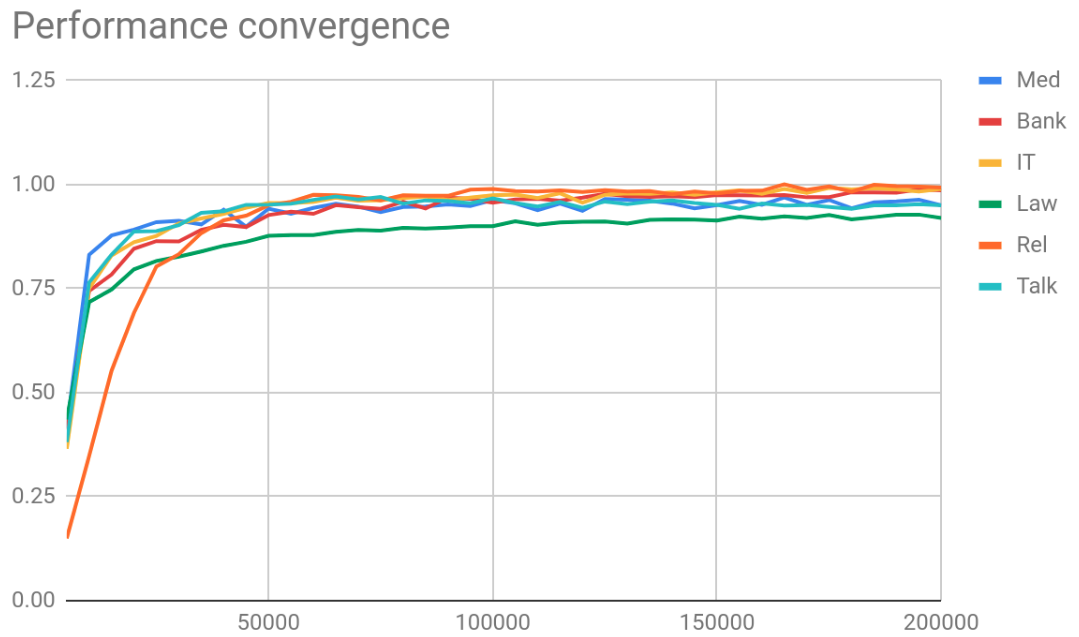
\includegraphics[width=\linewidth]{517.png}
\caption{MDMT performance in each domain under uniform sampling distribution}
\label{fig:uniform}
\end{figure}
Under uniform sampling distribution, the mdmt model received equivalent amounts of examples between domains. Figure \ref{fig:uniform} shows that with the same amount of training examples, the performance of the mdmt model approaches FT model's performance in the domains \domain{IT},\domain{bank} and \domain{rel} faster than in the domains \domain{law}, \domain{talk} and \domain{med}. We call domains having fast convergence "easy-domain", otherwise "hard-domain".

The different convergence rate between tasks was also reported in chapter 6 of \cite{Caruana97multitask}

By analyzing the sampling distribution optimized with DDS method, we observe that the resulting distribution is not optimal for harmonizing the heterogeneity of the convergence rate of the domains as an easy-domain such as \domain{rel} have same sampling probability as a hard-domain such as \domain{law}. A better sampling distribution should favor more the harder-domains such as \domain{med} and \domain{law}.

\subsection{Interpreting rewards via the proximity between domains (e.g vocabulary)}
Figure \ref{fig:reward} shows the trending lines of the rewards through the training course. We observe that the rewards of the domains do not have a large gap and they are very close to zero, that means a good domain between those domains simply does not hurt other domains.

Furthermore, the reward of a domain is simply the average of the cosine similarity between the gradient computed from a training batch sampled from that domain and each gradient computed from K dev sets. Reward may reveal the proximity between domains, therefore become a more natural way for instance weighing than such as Moore-Lewis score,
cosine similarity of sentence embedding, etc.

\begin{figure}[h!]
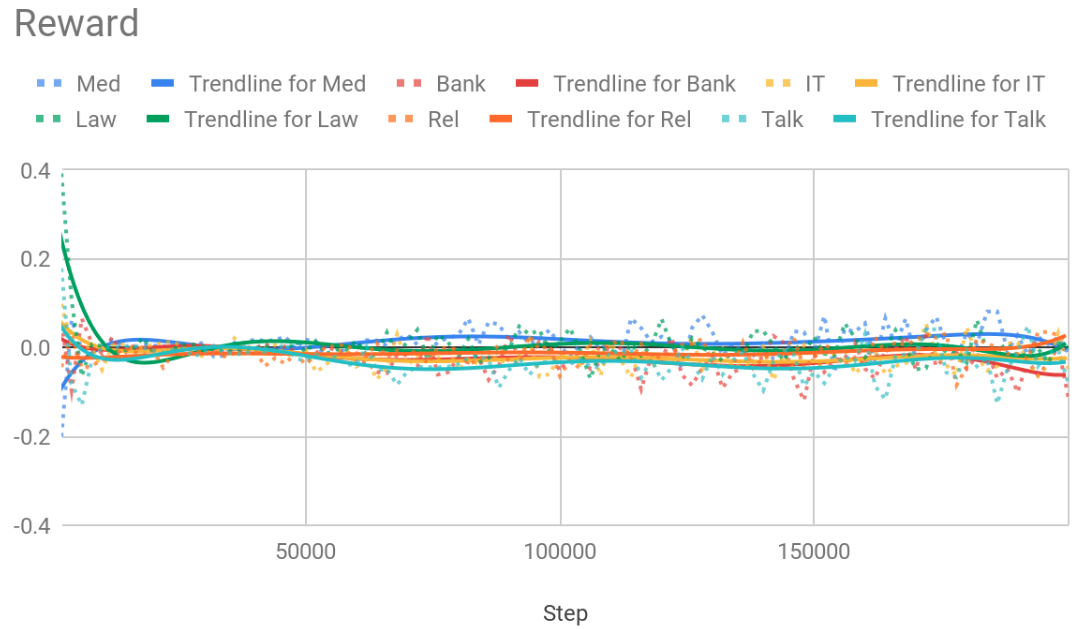
\includegraphics[width=\linewidth]{reward.png}
\caption{rewards of the domains}
\label{fig:reward}
\end{figure}

\section{Conclusion}
DDS method shows an excellent benefit in the domain adaptation problem as the method shows equivalent performance as fine-tuned mt system in the domain of interest while mitigate the significant drop in the other domains.

However, DDS method does not take in account the heterogeneity of the convergence rate of different domains which is also a key problem in mdmt training.
\bibliographystyle{acl_natbib}
\bibliography{multidomain}
\end{document}